\renewcommand{\NomeBloco}{Buffer}
\renewcommand{\NomePTab}{tab_\NomeBloco}
\renewcommand{\NomeSTab}{tab_\NomeBloco2}
\renewcommand{\NomePFig}{fig_\NomeBloco}
\renewcommand{\NomeSFig}{fig_\NomeBloco2}
\renewcommand{\NomeTTab}{tab_\NomeBloco3}

\section{\NomeBloco}
\label{inversor1}

O bloco \NomeBloco{} tem a finalidade de colocar o mesmo sinal de entrada na sua sa\'ida, reduzindo efeitos de carga. O sinal de entrada pode ser tanto anal\'ogico quanto digital. O bloco apresenta as defini{\c c}\~oes de sinais de entrada e sa\'ida referidos na \autoref{\NomeSTab}.

\begin{table}[htb]
\caption{Sinais do bloco \NomeBloco}
\label{\NomeSTab}
\centering
\begin{tabular}{ccl}

    \toprule
    Sinal & Tipo    & Descri{\c c}\~ao        \\
    \midrule \midrule
    In    & Entrada & Sinal de Entrada \\
    \midrule
    Out   & Saída   & Sinal de Sa\'ida   \\
    \bottomrule
\end{tabular}
\legend{Fonte: Produzido pelo autor}
\end{table}

O circuito projetado para o bloco \'e demonstrado na \autoref{\NomePFig}.

\begin{figure}[htb]
 \label{NomePFig}
 \centering
    \caption{Circuito CMOS projetado para o bloco \NomeBloco} \label{\NomePFig}
    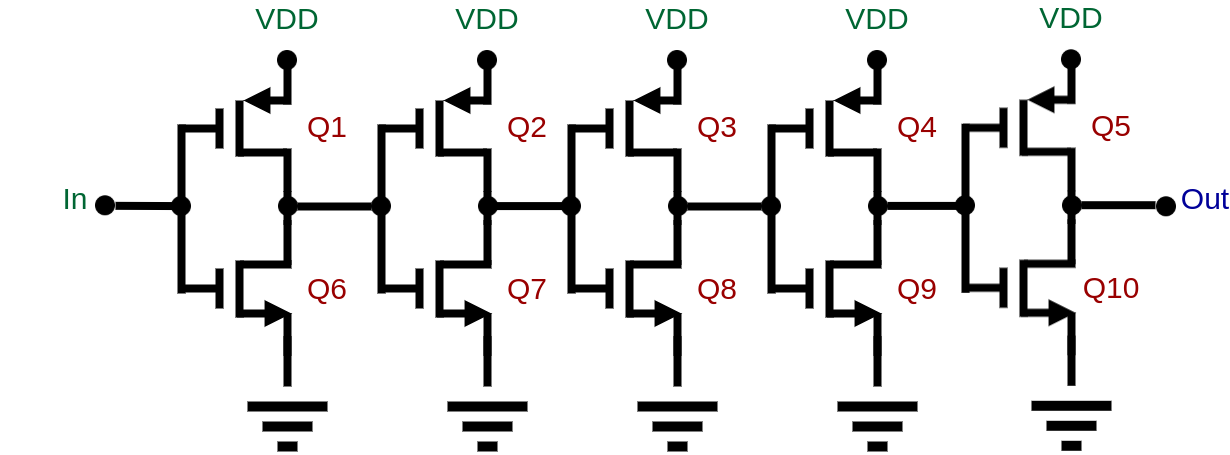
\includegraphics[scale=0.3]{Circuitos/Buffer.png}
    \legend{Fonte: Produzido pelo autor}
\end{figure}

\begin{figure}[htb]
 \label{NomePFig}
 \centering
    \centering
    \caption{Representa{\c c}\~ao em bloco do \NomeBloco} \label{NomeSFig2}
    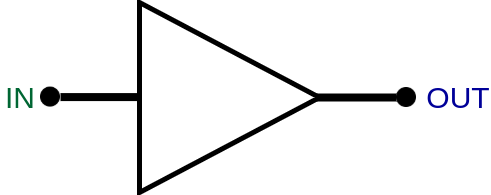
\includegraphics[scale=0.3]{Circuitos/Buffer_block.png}
    \legend{Fonte: Produzido pelo autor}
\end{figure}


Os transistores utilizados no bloco \NomeBloco{} apresentam os par\^ametros mostrados na \autoref{\NomeTTab}.

\begin{table}[htb]
\caption{Transistores do Bloco \NomeBloco}
\label{\NomeTTab}
\centering
\begin{tabular}{ccccc}
\toprule
Transistor & W ($\mu$m)  & L ($\mu$m)           & M (n° dispositivos) & S (n° dispositivos)\\
\midrule \midrule
Q1 e Q6 & 0,22 & 0,54 & 1 & 1\\
\midrule
Q2 e Q7 & 0,66 & 0,54 & 1 & 1\\
\midrule
Q3 e Q8 & 1,98 & 0,54 & 1 & 1\\
\midrule
Q4 e Q9 & 5,94 & 0,54 & 1 & 1\\
\midrule
Q5 e Q10 & 17,82 & 0,54 & 1 & 1\\
\bottomrule
\end{tabular}
\legend{Fonte: Produzido pelo autor}
\end{table}